\documentclass[10pt]{article}
\usepackage[a4paper,margin=1.5cm]{geometry}
\usepackage{graphicx,amssymb,amsmath}
\usepackage{array}
\usepackage{tikz}
\pagestyle{empty}
\setlength{\parindent}{0pt}

% the two A2 graphs on the 6 roots of a hexagon: 60-rule = hexagon, 120-rule = Star of David
\newcommand{\hexstar}{%
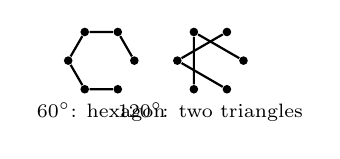
\begin{tikzpicture}[scale=0.42,dot/.style={circle,fill=black,inner sep=1.1pt},baseline=-2pt]
  \foreach \a in {0,...,5}{\node[dot](H\a) at (\a*60:1){};}
  \draw[thick](H0)--(H1)--(H2)--(H3)--(H4)--(H5)--cycle;
  \node[font=\scriptsize] at (0,-1.55) {$60^\circ$: hexagon};
  \begin{scope}[xshift=3.3cm]
    \foreach \a in {0,...,5}{\node[dot](S\a) at (\a*60:1){};}
    \draw[thick](S0)--(S2)--(S4)--cycle;
    \draw[thick](S1)--(S3)--(S5)--cycle;
    \node[font=\scriptsize] at (0,-1.55) {$120^\circ$: two triangles};
  \end{scope}
\end{tikzpicture}}

\newcommand{\thumb}[2]{%
  \begin{minipage}[t]{0.195\textwidth}\centering
    \includegraphics[width=\linewidth]{#1}\\[1pt]
    {\scriptsize #2}
  \end{minipage}}

\begin{document}

%================= PAGE 1 : THUMBNAILS =================
\begin{center}
  {\Large\bfseries The exceptional ladder --- orbital graphs}\\[2pt]
  {\small the basis of each Hecke algebra, drawn on its Coxeter plane}
\end{center}
\vspace{4pt}

{\bfseries E$_8$ rung \ --- \ $W(E_8)/W(E_7)$, 240 roots, rank-5 scheme}\\[4pt]
\thumb{e8_mandala.pdf}{$A$: ip $+1$, mandala = the $4_{21}$ polytope graph (56-reg)}\hfill
\thumb{e8_ip0.pdf}{$B$: ip $0$, bloom = orthogonality graph (126-reg)}\hfill
\thumb{e8_ipm1.pdf}{$C$: ip $-1$, weave = the $120^\circ$ twin (56-reg)}\hfill
\thumb{e8_ipm2.pdf}{$D$: ip $-2$, matching $120K_2$}\hfill
\begin{minipage}[t]{0.195\textwidth}\ \end{minipage}

\vspace{18pt}
{\bfseries E$_7$ rung \ --- \ $W(E_7)/W(E_6)$, 56 minuscule weights, rank-4 scheme}\\[4pt]
\thumb{e7_mandala.pdf}{$A$: ip $+1$, Gosset graph (27-reg)}\hfill
\thumb{e7_partner.pdf}{$B$: ip $0$, dist-2 graph of the Gosset graph (27-reg)}\hfill
\thumb{e7_bitangents.pdf}{$C$: ip $-1$, the 28 bitangents $28K_2$}\hfill
\begin{minipage}[t]{0.195\textwidth}\ \end{minipage}\hfill
\begin{minipage}[t]{0.195\textwidth}\ \end{minipage}

\vspace{14pt}
{\bfseries E$_6$ rung \ --- \ $W(E_6)/W(D_5)$, the 27 lines, rank-3 (strongly regular)}\\[4pt]
\thumb{e6_schlafli.pdf}{$A$: ip $0$, Schl\"afli graph $\mathrm{SRG}(27,10,1,5)$}\hfill
\thumb{e6_complement.pdf}{$B$: ip $+1$, Schl\"afli complement $\mathrm{SRG}(27,16,10,8)$}\hfill
\begin{minipage}[t]{0.195\textwidth}\ \end{minipage}\hfill
\begin{minipage}[t]{0.195\textwidth}\ \end{minipage}\hfill
\begin{minipage}[t]{0.195\textwidth}\ \end{minipage}

\vspace{14pt}
{\bfseries D$_5$ rung \ --- \ $W(D_5)/W(A_4)$, 16 half-spin weights, rank-3 (strongly regular)}\\[4pt]
\thumb{e5_clebsch.pdf}{$S$: ip $0$, Clebsch graph $\mathrm{SRG}(16,5,0,2)$}\hfill
\thumb{e5_halved5cube.pdf}{$T$: ip $+1$, halved 5-cube $\mathrm{SRG}(16,10,6,6)$}\hfill
\begin{minipage}[t]{0.195\textwidth}\ \end{minipage}\hfill
\begin{minipage}[t]{0.195\textwidth}\ \end{minipage}\hfill
\begin{minipage}[t]{0.195\textwidth}\ \end{minipage}

\vspace{12pt}
{\footnotesize All four are Gelfand pairs: the Hecke algebra
$\mathcal H(G,H)=\mathrm{End}_G\,\mathbb C[G/H]$ is commutative (a Bose--Mesner
algebra), with one basis element per inner-product class. These are
arc-transitive (Sabidussi) graphs. Multiplication and character (eigenvalue)
tables follow, one rung per page.}

\clearpage

%================= PAGE 2 : E8/E7 =================
\begin{center}{\Large\bfseries E$_8$ rung: $\ \mathcal H(W(E_8),W(E_7))$}\\[2pt]
{\small rank 5, basis $\{I,A,B,C,D\}$, valencies $1,56,126,56,1$}\end{center}
\vspace{10pt}

{\bfseries Multiplication table} \quad{\small(commutative; $I$ is the unit)}
\[
\renewcommand{\arraystretch}{1.2}
\begin{array}{c|ccccc}
\cdot & I & A & B & C & D\\\hline
A & A & 56I{+}27A{+}12B{+}C & 27A{+}32B{+}27C & A{+}12B{+}27C{+}56D & C\\
B & B & 27A{+}32B{+}27C & 126I{+}72A{+}60B{+}72C{+}126D & 27A{+}32B{+}27C & B\\
C & C & A{+}12B{+}27C{+}56D & 27A{+}32B{+}27C & 56I{+}27A{+}12B{+}C & A\\
D & D & C & B & A & I
\end{array}
\]
\vspace{4pt}

{\bfseries Character table} (the eigenmatrix $P$; row $i$ = eigenvalue of each
basis graph on eigenspace $i$; $m_i$ = multiplicity = $\dim$ of the paired
$W(E_8)$-module)
\[
\renewcommand{\arraystretch}{1.25}
\begin{array}{c|ccccc|l}
m_i & I & A & B & C & D & \text{module}\\\hline
1 & 1 & 56 & 126 & 56 & 1 & \mathbf 1\\
8 & 1 & 28 & 0 & -28 & -1 & \mathbf 8\ (\text{reflection rep})\\
35 & 1 & 8 & -18 & 8 & 1 & \mathbf{35}\\
112 & 1 & -2 & 0 & 2 & -1 & \mathbf{112}\\
84 & 1 & -4 & 6 & -4 & 1 & \mathbf{84}
\end{array}
\]
\vspace{2pt}

{\small $\mathcal H\cong\mathbb C^5$ (commutative, all irreps $1$-dimensional).
The grading element $D$ acts as $I\!\leftrightarrow\!D$, $A\!\leftrightarrow\!C$,
$B\!\mapsto\!B$ (the root antipode $r\mapsto-r$); its $\pm1$ eigenvalues (last
column) are the $\sigma$-even / $\sigma$-odd split. Folding by $D$ gives
$\mathrm{SRG}(120,56,28,24)$, whose spectrum is the three even rows.}

\vspace{10pt}
{\bfseries The five generators as rank-2 root subsystems}\\[2pt]
{\small Each generator is the $W(E_8)$-orbit of a pair of roots at a fixed
angle; that pair spans a rank-$\le2$ root subsystem. $E_8$ is simply-laced, so
only $A_1$, $A_1{\times}A_1$, $A_2$ can occur.}
\[
\renewcommand{\arraystretch}{1.35}
\begin{array}{r|ccccc}
\text{generator} & I & A & B & C & D\\\hline
\text{angle} & 0^\circ & 60^\circ & 90^\circ & 120^\circ & 180^\circ\\
\text{subsystem} & A_1 & A_2 & A_1{\times}A_1 & A_2 & A_1\\
\text{diagram} & \circ & \circ\!\!-\!\!\circ & \circ\ \ \circ & \circ\!\!-\!\!\circ & \circ
\end{array}
\]
{\small The Dynkin label is $5\!\to\!3$: it sees the angle only up to the
subsystem's own Weyl group, merging $I,D$ (both $A_1$) and $A,C$ (both $A_2$).
The missing bit is \emph{orientation} --- and orientation-reversal is exactly
the grading $D$, which swaps $A\!\leftrightarrow\!C$, $I\!\leftrightarrow\!D$
and fixes the orientation-symmetric $B=A_1{\times}A_1$.}

\vspace{8pt}
\begin{center}\fbox{\parbox{0.93\textwidth}{\small
\textbf{Remark --- the two $A_2$ graphs.} $A$ ($60^\circ$) and $C$ ($120^\circ$)
are \emph{both} of type $A_2$, yet they are different graphs on the same roots.
The reason is visible on the six roots of a single $A_2$ (a hexagon of roots):
the $60^\circ$ rule gives the hexagon (a $6$-cycle), the $120^\circ$ rule gives
the two triangles (Star of David) --- the $120^\circ$ neighbours are the
antipodes of the $60^\circ$ neighbours. The mandala $A$ and the weave $C$ are
exactly this picture scaled to $240$ roots: the same points, the two
$A_2$-relations, related by the antipode $r\mapsto-r$ but \emph{not equal}.
\\[4pt]\centerline{\hexstar}}}\end{center}

\clearpage

%================= PAGE 3 : E7/E6 =================
\begin{center}{\Large\bfseries E$_7$ rung: $\ \mathcal H(W(E_7),W(E_6))$}\\[2pt]
{\small rank 4, basis $\{I,A,B,C\}$, valencies $1,27,27,1$}\end{center}
\vspace{10pt}

{\bfseries Multiplication table} \quad{\small(commutative; $I$ is the unit)}
\[
\renewcommand{\arraystretch}{1.4}
\begin{array}{c|cccc}
\cdot & I & A & B & C\\\hline
A & A & 27I{+}16A{+}10B & 10A{+}16B{+}27C & B\\
B & B & 10A{+}16B{+}27C & 27I{+}16A{+}10B & A\\
C & C & B & A & I
\end{array}
\]
\vspace{4pt}

{\bfseries Character table} (eigenmatrix $P$; $m_i$ = multiplicity = $\dim$ of
the paired $W(E_7)$-module)
\[
\renewcommand{\arraystretch}{1.25}
\begin{array}{c|cccc|l}
m_i & I & A & B & C & \text{module}\\\hline
1 & 1 & 27 & 27 & 1 & \mathbf 1\\
7 & 1 & 9 & -9 & -1 & \mathbf 7\ (\text{reflection rep})\\
27 & 1 & -1 & -1 & 1 & \mathbf{27}\\
21 & 1 & -3 & 3 & -1 & \mathbf{21}
\end{array}
\]
\vspace{2pt}

{\small $\mathcal H\cong\mathbb C^4$ (commutative). The antipode $C$ acts as
$I\!\leftrightarrow\!C$, $A\!\leftrightarrow\!B$ (the matching $w\mapsto r_0-w$),
forcing $A^2=B^2$. Folding by $C$ collapses the Gosset graph to the complete
graph $K_{28}$ (the two $\sigma$-even rows, $m_i=1,27$, are exactly the spectrum
of $K_{28}$).

\smallskip
The ordering $I,A,B,C$ is the \emph{distance ordering} of the Gosset graph
$A$: the table entry $A^2=27I+16A+10B$ has a $B$ term but \emph{no} $C$ term,
so a $B$-pair has $10$ common neighbours (distance $2$) while a $C$-pair has
none (distance $3$, the graph being connected of diameter $3$). Hence $B$ is the
\textbf{distance-$2$ graph of the Gosset graph} and $C$ its distance-$3$ graph.
This needs no separate proof --- it is read off the multiplication table
($B=(A^2-27I-16A)/10$ is a degree-$2$ polynomial in $A$); $B$ is itself
distance-transitive, the catalogued graph with intersection array
$\{27,16,1;1,16,27\}$.}

\vspace{10pt}
{\bfseries The four generators as rank-2 root subsystems}\\[2pt]
{\small The $56$ weights are themselves $E_8$ roots, so each pair again spans an
$A_1$, $A_1{\times}A_1$ or $A_2$.}
\[
\renewcommand{\arraystretch}{1.35}
\begin{array}{r|cccc}
\text{generator} & I & A & B & C\\\hline
\text{angle} & 0^\circ & 60^\circ & 90^\circ & 120^\circ\\
\text{subsystem} & A_1 & A_2 & A_1{\times}A_1 & A_2\\
\text{diagram} & \circ & \circ\!\!-\!\!\circ & \circ\ \ \circ & \circ\!\!-\!\!\circ
\end{array}
\]

\vspace{6pt}
\begin{center}\fbox{\parbox{0.93\textwidth}{\small
\textbf{Note --- the two equal-degree graphs and their angles.}
In the \textbf{E$_8$ rung} the two $56$-regular generators $A,C$ lie at
$\mathbf{60^\circ}$ and $\mathbf{120^\circ}$: \emph{both} of type $A_2$,
exchanged by the central-inversion grading $D$ (same diagram, reversed
orientation). In the \textbf{E$_7$ rung} the two $27$-regular generators $A,B$
lie at $\mathbf{60^\circ}$ and $\mathbf{90^\circ}$: of \emph{different} types
$A_2$ and $A_1{\times}A_1$. Their equal valency is not an orientation symmetry
but a genuine coincidence of the scheme, and the affine grading $w\mapsto r_0-w$
carries one type into the other. (In the E$_6$ rung below, the $60^\circ$ and
$90^\circ$ graphs instead have \emph{different} degrees $16$ and $10$: the
complement is $A_2$, the Schl\"afli graph is $A_1{\times}A_1$.)}}\end{center}

\vspace{8pt}
\begin{center}\fbox{\parbox{0.93\textwidth}{\small
\textbf{Remark --- the two $A_2$ graphs.} E$_7$ also carries both $A_2$
relations, $A$ ($60^\circ$) and $C$ ($120^\circ$) --- but here they are wildly
different sizes: the $60^\circ$ one is the full Gosset graph ($27$-regular), the
$120^\circ$ one is just the valency-$1$ antipodal matching $w\mapsto r_0-w$. The
hexagon-vs-Star-of-David reason is the same as for E$_8$: on the six roots of
one $A_2$, the $60^\circ$ rule gives the hexagon, the $120^\circ$ rule the two
triangles.
\\[4pt]\centerline{\hexstar}}}\end{center}

\clearpage

%================= PAGE 4 : E6/D5 =================
\begin{center}{\Large\bfseries E$_6$ rung: $\ \mathcal H(W(E_6),W(D_5))$}\\[2pt]
{\small rank 3, basis $\{I,A,B\}$, valencies $1,10,16$;
$A=$ Schl\"afli, $B=$ complement}\end{center}
\vspace{10pt}

{\bfseries Multiplication table} \quad{\small(commutative; $I$ is the unit)}
\[
\renewcommand{\arraystretch}{1.4}
\begin{array}{c|ccc}
\cdot & I & A & B\\\hline
A & A & 10I{+}A{+}5B & 8A{+}5B\\
B & B & 8A{+}5B & 16I{+}8A{+}10B
\end{array}
\]
The relation $A^2=10I+A+5B$ is the defining equation of the strongly regular
graph $\mathrm{SRG}(27,10,1,5)$ ($\lambda=1$, $\mu=5$); likewise
$B^2=16I+8A+10B$ for $\mathrm{SRG}(27,16,10,8)$.
\vspace{6pt}

{\bfseries Character table} (eigenmatrix $P$; $m_i$ = multiplicity = $\dim$ of
the paired $W(E_6)$-module)
\[
\renewcommand{\arraystretch}{1.25}
\begin{array}{c|ccc|l}
m_i & I & A & B & \text{module}\\\hline
1 & 1 & 10 & 16 & \mathbf 1\\
20 & 1 & 1 & -2 & \mathbf{20}\\
6 & 1 & -5 & 4 & \mathbf 6\ (\text{reflection rep})\\
\end{array}
\]
\vspace{2pt}

{\small $\mathcal H\cong\mathbb C^3$ (commutative, strongly regular). This is the
bottom of the ladder: $27$ is odd, so there is \emph{no} antipodal matching and
no grading element --- the rung is \emph{terminal} and cannot fold further. The
reflection representation $\mathbf 6$ (eigenvalue $-5$ on Schl\"afli) completes
the rank descent $\mathbf 8\!\to\!\mathbf 7\!\to\!\mathbf 6$ of the three
reflection reps down the ladder.}

\vspace{10pt}
{\bfseries The three generators as rank-2 root subsystems}\\[2pt]
{\small The $27$ lines are $E_8$ roots too; with no $120^\circ$ class the scheme
reaches only $A_2$ and $A_1{\times}A_1$.}
\[
\renewcommand{\arraystretch}{1.35}
\begin{array}{r|ccc}
\text{generator} & I & A\ (\text{Schl\"afli}) & B\ (\text{complement})\\\hline
\text{angle} & 0^\circ & 90^\circ & 60^\circ\\
\text{subsystem} & A_1 & A_1{\times}A_1 & A_2\\
\text{diagram} & \circ & \circ\ \ \circ & \circ\!\!-\!\!\circ
\end{array}
\]

\vspace{6pt}
\begin{center}\fbox{\parbox{0.93\textwidth}{\small
\textbf{Remark --- only one $A_2$ here.} Unlike E$_8$ and E$_7$, the E$_6$ rung
has \emph{no} $120^\circ$ class, so it carries only the single $A_2$ graph (the
$60^\circ$ complement) --- there is no Star-of-David partner. That missing
$120^\circ$ twin is the geometric face of the same fact seen algebraically
above: $27$ is odd, there is no antipodal matching, and the rung is
\emph{terminal}.}}\end{center}

\clearpage

%================= PAGE 5 : D5/A4 =================
\begin{center}{\Large\bfseries D$_5$ rung: $\ \mathcal H(W(D_5),W(A_4))$}\\[2pt]
{\small rank 3, basis $\{I,S,T\}$, valencies $1,5,10$;
$S=$ Clebsch graph, $T=$ halved $5$-cube}\end{center}
\vspace{10pt}

{\bfseries Multiplication table} \quad{\small(commutative; $I$ is the unit)}
\[
\renewcommand{\arraystretch}{1.4}
\begin{array}{c|ccc}
\cdot & I & S & T\\\hline
S & S & 5I{+}2T & 4S{+}3T\\
T & T & 4S{+}3T & 10I{+}6S{+}6T
\end{array}
\]
The relation $S^2=5I+2T$ is the defining equation of the Clebsch graph
$\mathrm{SRG}(16,5,0,2)$ ($\lambda=0$, $\mu=2$, the folded $5$-cube); likewise
$T^2=10I+6S+6T$ for its complement $\mathrm{SRG}(16,10,6,6)$, the halved
$5$-cube.
\vspace{6pt}

{\bfseries Character table} (eigenmatrix $P$; $m_i$ = multiplicity = $\dim$ of
the paired $W(D_5)$-module)
\[
\renewcommand{\arraystretch}{1.25}
\begin{array}{c|ccc|l}
m_i & I & S & T & \text{module}\\\hline
1 & 1 & 5 & 10 & \mathbf 1\\
10 & 1 & 1 & -2 & \mathbf{10}\\
5 & 1 & -3 & 2 & \mathbf 5\ (\text{reflection rep})\\
\end{array}
\]
\vspace{2pt}

{\bfseries The three generators as rank-2 root subsystems}\\[2pt]
{\small Like E$_6$, with no $120^\circ$ class the scheme reaches only $A_2$ and
$A_1{\times}A_1$.}
\[
\renewcommand{\arraystretch}{1.35}
\begin{array}{r|ccc}
\text{generator} & I & S\ (\text{Clebsch}) & T\ (\text{halved 5-cube})\\\hline
\text{angle} & 0^\circ & 90^\circ & 60^\circ\\
\text{subsystem} & A_1 & A_1{\times}A_1 & A_2\\
\text{diagram} & \circ & \circ\ \ \circ & \circ\!\!-\!\!\circ
\end{array}
\]
\vspace{2pt}

{\small $\mathcal H\cong\mathbb C^3$ (commutative, strongly regular), terminal
like E$_6$: $16$ carries no antipodal matching into the scheme, so there is no
grading element and no fold. The reflection representation $\mathbf 5$
(eigenvalue $-3$ on the Clebsch graph) continues the rank descent
$\mathbf 8\!\to\!\mathbf 7\!\to\!\mathbf 6\!\to\!\mathbf 5$.}

\vspace{14pt}
{\footnotesize\itshape Note. The four rungs above are the one-step (minuscule)
descents $E_8\supset E_7\supset E_6\supset D_5$, all Gelfand pairs; the rank-3
rungs hand back the classical SRGs Schl\"afli and Clebsch, and one further step
$W(A_4)/W(A_3{\times}A_1)$ gives the Petersen graph before the series goes
reducible. Skipping a rung instead --- $W(E_8)/W(E_6)$, the $13440$ flags of two
roots at $60^\circ$ --- is \emph{not} a Gelfand pair: that Hecke algebra has
dimension $79$ and is non-commutative,
$\mathbb C^7\oplus M_2(\mathbb C)^5\oplus M_3(\mathbb C)^4\oplus M_4(\mathbb C)$,
because $W(E_6)$ fixes the $2$-plane $\langle r_0,w_0\rangle$ and so doubles the
reflection representation.}

\end{document}
